Bu kısmına kadar yapılan süreç ortalaması ve süreç standart sapması hakkındaki yorumlamalardan sonra artık yeni soru hakkında yorumlamalar yapılacaktır.\\

İlk öncelikle gözlemlenen ağırlıkların histogram grafiğini çizelim. 

\begin{center}
	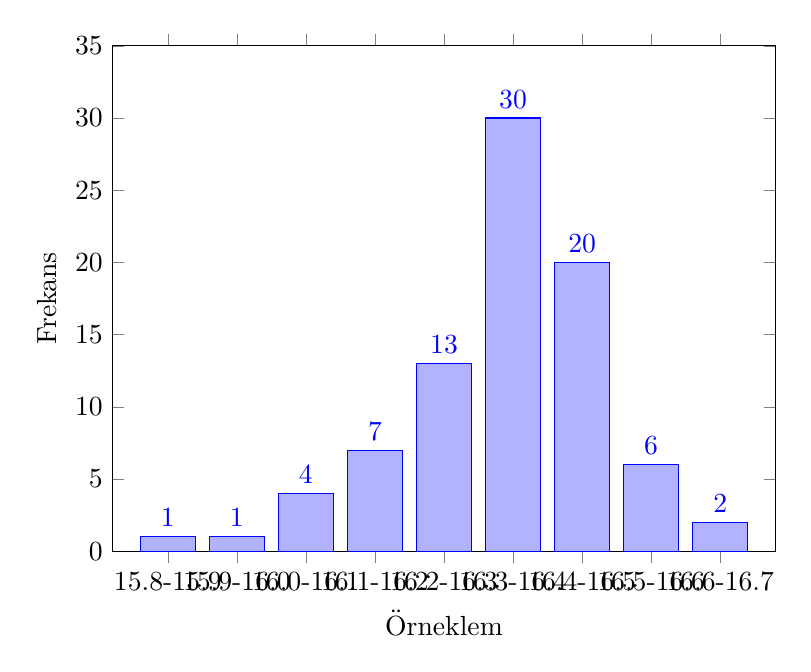
\begin{tikzpicture}
		\begin{axis}[
			ybar,
			bar width=0.7cm,
			width=10cm,
			height=8cm,
			xlabel={Örneklem},
			ylabel={Frekans},
			symbolic x coords={15.8-15.9, 15.9-16.0, 16.0-16.1, 16.1-16.2, 16.2-16.3, 16.3-16.4, 16.4-16.5, 16.5-16.6, 16.6-16.7},
			xtick=data,
			nodes near coords,
			ymin=0,
			ymax=35
			]
			\addplot coordinates {
				(15.8-15.9, 1)
				(15.9-16.0, 1)
				(16.0-16.1, 4)
				(16.1-16.2, 7)
				(16.2-16.3, 13)
				(16.3-16.4, 30)
				(16.4-16.5, 20)
				(16.5-16.6, 6)
				(16.6-16.7, 2)
			};
		\end{axis}
	\end{tikzpicture}
\end{center}

Süreç boyunca kaydedilen tüm ağırlıkların normal dağılıma sahip olduğunu anlamanın en basit yolu histogram grafiğinin çan eğrisi ile kıyaslamaktır. Bu, dağılımın normal olup olmadığını anlamamız için şimdilik yeterlidir. Histograma göre söylenebilir ki evet, veriler normal dağılıma yakındırlar.

